% headsectionstart
% update mixedReport hedsection if any changes done in this headsection
\documentclass{article}
\usepackage[a4paper, left=15pt, top=30pt, right=15pt, bottom=65pt]{geometry}
\usepackage{longtable}
\usepackage[table]{xcolor}
\usepackage{graphicx}
\usepackage{tikz}
\usepackage{atbegshi}
\usepackage{adjustbox}
\usepackage[sfdefault]{roboto}
\usepackage[T1]{fontenc}
\usepackage{minted}
\usepackage[colorlinks = true,
linkcolor = blue,
urlcolor  = blue,
citecolor = blue,
anchorcolor = blue]{hyperref}

\usetikzlibrary{fit,backgrounds,positioning,decorations.markings,shapes,arrows,shadows}
\definecolor{primary}{RGB}{115,54,163}
\definecolor{theftBgColor1}{RGB}{235,215,249}
\definecolor{theftBgColor2}{RGB}{238,229,197}
\definecolor{theftValueType1Color}{RGB}{0,0,0}
\definecolor{theftValueType2Color}{RGB}{115,54,163}
\definecolor{theftValueType3Color}{RGB}{125,110,142}
\definecolor{yesVoteColor}{RGB}{115,54,163}
\definecolor{noVoteColor}{RGB}{61,38,80}
\definecolor{yesNoBarBgColor}{HTML}{EDEDED}
\definecolor{yesNoBarBorderColor}{HTML}{B2AEAE}
\definecolor{noProgressBgColor}{HTML}{E26C6C}
\definecolor{tableHeaderBg}{HTML}{F0EAFA}
\definecolor{oddRowColor}{HTML}{F1F4F6}
\definecolor{evenRowColor}{HTML}{FAFCFD}

\tikzset{
	headerText/.style={text=white},
	leftHeaderText/.style={headerText, align=left,text width=280pt},
	rightHeaderText/.style={headerText, align=right,text width=225pt},
	footerText/.style={text=white},
	leftFooterText/.style={footerText, align=left,text width=380pt},
	rightFooterText/.style={footerText, align=right,text width=193pt},
	fullWidth/.style={text width=535pt},
  yesNoBar/.style={minimum width=101pt, minimum height=30pt},
	yesNoBarBg/.style={yesNoBar, draw=yesNoBarBorderColor, fill=yesNoBarBgColor, rounded corners=3pt, line width=1pt, right},
	yesNoBarProgress/.style={yesNoBar, fill=primary, minimum height=29pt, rounded corners=2.5pt, right= -101.25pt, inner sep=0},
	yesNoBarText/.style={yesNoBar, right, white, right= -101.25pt},
	theftBlock/.style={rounded corners=5pt, inner sep=10pt},
	theftBlockContent/.style={text=black, text width=100pt},
	isTheftBlock/.style={align=left, text width=140pt}
}

\newcommand\Footer{%
  \sffamily
  \begin{tikzpicture}[remember picture,overlay]
    \node[leftFooterText] at (124pt, -734pt) (leftTop) {\Large Amount taken unethically from citizens in a rigged economy};
    \node[leftFooterText, below=-3pt of leftTop] (leftBottom) {Numbers and Theft vs. not Theft come from citizen voting
    and not ZTM Technologies SPC or this website};

    \node[rightFooterText, right=5pt of leftTop] (calculated) {--generatedTime-- \quad Page \thepage};
    \node[rightFooterText, below=0pt of calculated] (generatedBy) {Generated By \href{--holonUrl--}{\color{white}--holonUrl--}};

    \begin{scope}[on background layer]
    \node[fill=primary, fit=(leftTop)(leftBottom)(calculated)(generatedBy)] (footer) {};
    \end{scope}
  \end{tikzpicture}%
}

\pagestyle{empty}
\AtBeginShipout{\AtBeginShipoutAddToBox{\Footer}}

\begin{document}
\sffamily
% headsectionend

\hypertarget{--pageID--}{}
% header
\trimbox{0 -15pt 0 0}{ 
  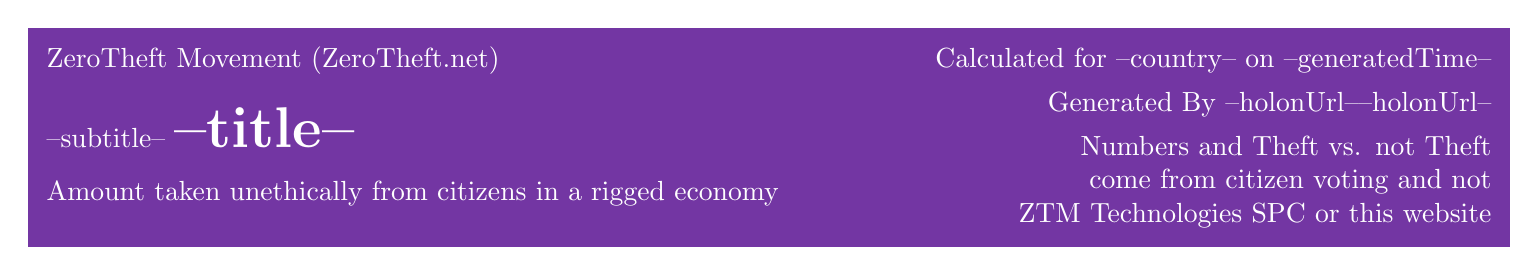
\begin{tikzpicture}
      \node[leftHeaderText] (top) {ZeroTheft Movement (ZeroTheft.net)};
      \node[leftHeaderText, below=5pt of top] (title) {--subtitle-- \huge \textbf{--title--}};
      \node[leftHeaderText, below=5pt of title] (belowtitle) {Amount taken unethically from citizens in a rigged economy};

      \node[rightHeaderText, right=10pt of top] (calculated) {Calculated for --country-- on --generatedTime--};
      \node[rightHeaderText, below=0pt of calculated] (generatedBy) {Generated By \href{--holonUrl--}{\color{white}--holonUrl--}};
      \node[rightHeaderText, below=0pt of generatedBy] (truth) {
        Numbers and Theft vs. not Theft come from citizen voting
        and not ZTM Technologies SPC or this website
      };
    
      \begin{scope}[on background layer]
      \node[fill=primary, fit=(top)(title)(belowtitle)(calculated)(generatedBy)(truth)] (header) {};
      \end{scope}
  \end{tikzpicture}
}

\trimbox{-136pt -15pt 0 0}{ 
  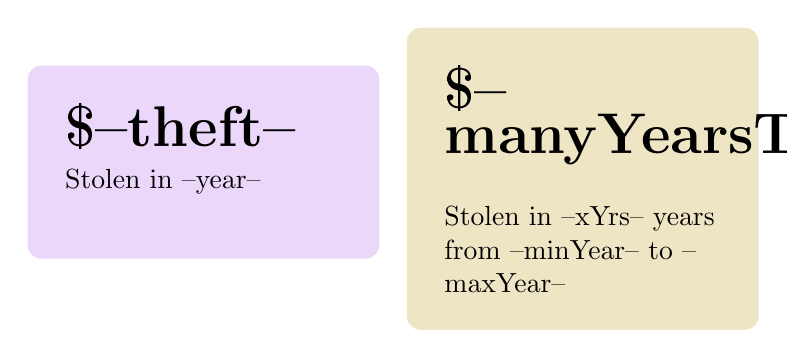
\begin{tikzpicture}
      \node[theftBlockContent] (amount1) {\huge \textbf{\$--theft--}};
      \node[theftBlockContent, below=0ptof amount1] (year1) {Stolen in --year--\newline};
      
      \begin{scope}[on background layer]
      \node[theftBlock, fill=theftBgColor1, fit=(amount1)(year1)] (block1) {};
      \end{scope}

      \node[theftBlockContent, right=30ptof amount1] (amount2) {\huge \textbf{\$--manyYearsTheft--}};
      \node[theftBlockContent, below=0ptof amount2] (year2) {Stolen in --xYrs-- years\\from --minYear-- to --maxYear--};
      
      \begin{scope}[on background layer]
      \node[theftBlock, fill=theftBgColor2, fit=(amount2)(year2)] (block2) {};
      \end{scope}
  \end{tikzpicture}
}

\trimbox{25pt -20pt 0 0}{
  \begin{tikzpicture}
    % \node[] (theftValueChart) {\includegraphics[width=565pt]{/Volumes/WorkSpace/WhiteHat/zerotheft/zerotheft-holon-node/zt_report/reports/ztReport/USA-tax-corp_tax_evasion-theftValue.png}};
    \node[] (theftValueChart) {\includegraphics[width=565pt]{--theftValueChart--}};
  \end{tikzpicture}
}

% yesNoBlockStart
\trimbox{0 -20pt 0 0}{
  \begin{tikzpicture}
    \node[isTheftBlock, primary] (isTheft) {\LARGE \textbf{IS THIS THEFT?}};
    \node[below=1pt of isTheft, isTheftBlock] (noOfVoters) {\large Total No of Voters:};
    \node[below=0pt of noOfVoters, isTheftBlock] (noOfVotersNum) {\LARGE \textbf{--totalVotes--}};
    \node[below=10pt of noOfVotersNum, isTheftBlock] (votedYes) {\large Voted Yes: --yesVotes--};
    \node[below=0pt of votedYes, isTheftBlock] (votedNo) {\large Voted No: --noVotes--};
    
    % \node[yshift=-40pt, right=-10pt of isTheft] (noVoteImage) {\includegraphics[width=120pt]{/Volumes/WorkSpace/WhiteHat/zerotheft/zerotheft-holon-node/zt_report/reports/ztReport/USA-tax-corp_tax_evasion-yesNo.png}};
    \node[yshift=-40pt, right=-10pt of isTheft] (noVoteImage) {\includegraphics[width=120pt]{--yesNoChart--}};
  \end{tikzpicture}
}
% yesNoBlockEnd
% votesForTheftAllYearsBlockStart
\trimbox{3pt 15pt 0 0}{
  \begin{tikzpicture}
    % \node[] (theftValueChart) {\includegraphics[width=270pt]{/Volumes/WorkSpace/WhiteHat/zerotheft/zerotheft-holon-node/zt_report/reports/ztReport/USA-tax-corp_tax_evasion-votesForTheftAmount.png}};
    \node[] (theftValueChart) {\includegraphics[width=270pt]{--votesForTheftAmountChart--}};
  \end{tikzpicture}
}
% votesForTheftAllYearsBlockEnd

% votesForTheft5yearsBlockStart
\trimbox{8pt -10pt 0 0}{
  \begin{tikzpicture}
    % \node[] (theftValueChart) {\includegraphics[width=270pt]{/Volumes/WorkSpace/WhiteHat/zerotheft/zerotheft-holon-node/zt_report/reports/ztReport/USA-tax-corp_tax_evasion-votesForTheftAmount.png}};
    \node[] (theftValueChart) {\includegraphics[width=270pt]{--votesForTheftAmountFiveYearsAgoChart--}};
  \end{tikzpicture}
}
% votesForTheft5yearsBlockEnd
% votesForTheftLastYearBlockStart
\trimbox{8pt -10pt 0 0}{
  \begin{tikzpicture}
    % \node[] (theftValueChart) {\includegraphics[width=270pt]{/Volumes/WorkSpace/WhiteHat/zerotheft/zerotheft-holon-node/zt_report/reports/ztReport/USA-tax-corp_tax_evasion-votesForTheftAmount.png}};
    \node[] (theftValueChart) {\includegraphics[width=270pt]{--votesForTheftAmountLastYearChart--}};
  \end{tikzpicture}
}
% votesForTheftLastYearBlockEnd

\setlength{\tabcolsep}{8pt} % for the horizontal padding
{\renewcommand{\arraystretch}{2}% for the vertical padding
  \begin{longtable}{p{16pt} p{38pt} p{16pt} p{38pt} p{16pt} p{38pt} p{0pt} p{16pt} p{38pt} p{16pt} p{38pt} p{16pt} p{38pt}} 
    \rowcolor{primary}
    \multicolumn{6}{l}{\color{white} Not Translated into --inflationYear-- Dollar Values} & \cellcolor{white} &
    \multicolumn{6}{l}{\color{white} Translated into --inflationYear-- Dollar Values} \\ 

    --stolenByYearTableData--
    % \rowcolor{oddRowColor} 8888 & \$888.88B & 2019 & \$650B & 2019 & \$888.88B & \cellcolor{white} & 2021 & \$800B & 2019 & \$701B & 2019 & \$650B \\
    % \rowcolor{evenRowColor} 2020 & \$700B & 2018 & \$600B & 2019 & \$650B & \cellcolor{white} & 2020 & \$725B & 2018 & \$656B & 2019 & \$650B \\
\end{longtable}
}

% proposalYamlBlockStart
\newpage 
\trimbox{0 10pt 0 0}{ 
  
\begin{tikzpicture}
    \node[fullWidth, text=primary] (leadingProposal) {\huge \textbf{Leading Proposals}};
    \node[fullWidth, below =0ptof leadingProposal] (viewProposalTextLink) {\href{--holonUrl--/path/--pathSlug--/issue/--leafSlug--}{\color{blue}View Full Proposal Text}};
    \node[fullWidth, below =0ptof viewProposalTextLink] (leadingProposalTitle) {\large \textbf{Proposal by --leadingProposalAuthor-- on --leadingProposalDate--}};
  \end{tikzpicture}
}

\noindent
  \begin{minted}[%
    breaklines,
    mathescape,
    numbersep=5pt,
    numbersep=5pt,
    xleftmargin=30pt,
    xrightmargin=30pt,
    breaksymbolleft=,
    gobble=0,
    linenos
  ]{yaml}
--leadingProposalDetail--
  \end{minted}

  --viewMore--
% proposalYamlBlockEnd
\end{document}
